\documentclass[12pt]{article}

% ------------------------------------------------------------------
% Formatting: Times New Roman, US Letter, margins, double-spaced
% ------------------------------------------------------------------
\usepackage[letterpaper, top=1.5in, bottom=1.5in, left=1in, right=1in]{geometry}
\usepackage[T1]{fontenc}
\usepackage[utf8]{inputenc}
\usepackage{mathptmx}          % Times New Roman
\usepackage{setspace}
\doublespacing

\usepackage{amsmath,amssymb}
\usepackage{booktabs}
\usepackage{graphicx}
\usepackage{float}
\usepackage{caption}
\usepackage[round]{natbib}
\usepackage{hyperref}
\usepackage{array}

\graphicspath{{../output/figures/}}

\hypersetup{
    colorlinks=true,
    linkcolor=black,
    citecolor=black,
    urlcolor=black
}

% ------------------------------------------------------------------
\begin{document}

% ==================================================================
% TITLE PAGE
% ==================================================================
\begin{center}
{\LARGE \textbf{Factor Investing in Emerging Markets}} \\[1.5em]
{\large Andy Zhang \quad Coco Dong \quad Scarlett He \quad Yanni Zheng} \\[0.8em]
{\normalsize Columbia Business School} \\[0.8em]
{\normalsize \today}
\end{center}

\vspace{1.5em}

% ==================================================================
% ABSTRACT
% ==================================================================
\begin{center}
\textbf{Abstract}
\end{center}

\begin{quote}
\noindent
We evaluate a systematic multi-factor strategy for emerging market equities using six stock-level characteristics across eleven industries over 2004--2025. Equal-weighting all six factors into a composite score dominates more complex alternatives out-of-sample (Sharpe ratio 0.44). Momentum-weighted cross-industry allocation further improves performance (Sharpe 0.59). Dynamic beta hedging against the MSCI EM Index produces a market-neutral strategy with Sharpe ratio of 1.47, annualized alpha of 8.9\%, and maximum drawdown of 7.2\%. The strategy is robust under country-weighted transaction costs of 45 basis points (net Sharpe 1.30), generates positive alpha in both rising and falling EM markets, and has break-even costs of 127 basis points.
\end{quote}

\vspace{0.5em}
\noindent\textit{Keywords:} Factor investing, emerging markets, multi-factor portfolios, portfolio construction, beta hedging, information coefficient

\noindent\textit{JEL Classification:} G11, G12, G15

\newpage

% ==================================================================
% 1. INTRODUCTION
% ==================================================================
\section{Introduction}

Factor investing---the systematic exploitation of cross-sectional return predictability based on observable stock characteristics---has transformed modern quantitative asset management. While the literature on factor premia in developed markets is extensive \citep{famafrench1993, famafrench2015, carhart1997}, evidence from emerging markets (EM) remains comparatively limited. This gap is economically significant: EM equities account for a substantial share of global market capitalization, and their lower analyst coverage, weaker information efficiency, and greater institutional frictions may offer richer opportunities for systematic strategies \citep{cakici2013, hanauer2015, hou2011}.

This paper investigates four interconnected questions. First, which of the canonical stock-level characteristics---size, value, quality, momentum, volatility, and dividend yield---predict cross-sectional returns across EM industries, and how stable is their predictive power over time? Second, how should multiple factor signals be combined into a composite stock selection score---does complex optimization outperform simple equal weighting? Third, which cross-industry portfolio construction technique delivers the best risk-adjusted performance? Fourth, can dynamic beta hedging isolate a robust, market-neutral alpha stream that survives realistic transaction costs?

We address these questions using a comprehensive sample of 98,742 stock-month observations spanning 953 unique stocks across 15 EM countries and 255 months (January 2004 to March 2025). Our research pipeline proceeds sequentially: we first evaluate factor information coefficients (ICs) within each of eleven GICS-based industries, then compare eight multi-factor composition methods, apply ten cross-industry portfolio construction techniques, and finally implement dynamic beta hedging with transaction cost analysis.

Our principal findings are as follows. First, all six factors carry cross-sectional predictive information in EM, with size and value (price-to-book) exhibiting the strongest and most consistent ICs, though the sign of the value premium is reversed relative to developed markets---high P/B stocks outperform. Second, naively equal-weighting all six factors (``All6-EW'') achieves the highest out-of-sample Sharpe ratio (0.44 over 2014--2025) among eight composition methods, consistent with the finding of \citet{demiguel2009} that estimation error renders simple diversification preferable to optimization. Third, momentum-weighted cross-industry allocation outperforms nine alternative techniques with a Sharpe ratio of 0.59. Fourth, dynamic beta hedging transforms this moderate long-only strategy into a market-neutral alpha stream with a Sharpe ratio of 1.47, annualized alpha of 8.9\%, maximum drawdown of 7.2\%, and positive alpha in both rising and falling EM environments. Under country-weighted transaction costs of 45 bps the net Sharpe remains 1.30, and the break-even for Sharpe $> 1.0$ is 127 basis points.

The remainder of this paper is organized as follows. Section~2 reviews the related literature. Section~3 describes the data. Section~4 presents the empirical analysis and results. Section~5 addresses robustness. Section~6 concludes.


% ==================================================================
% 2. LITERATURE REVIEW
% ==================================================================
\section{Literature Review}

\paragraph{Factor premia and emerging markets.} The modern factor literature originates with \citet{famafrench1993}, who document the size and value premia in U.S.\ equities. \citet{carhart1997} adds momentum, establishing the four-factor benchmark, while \citet{novymarx2013} identifies profitability and \citet{famafrench2015} formalizes the five-factor model. \citet{ang2006} document the low-volatility anomaly. \citet{harvey2016}, surveying over 300 published factors, raise the bar for statistical significance by highlighting the pervasiveness of data mining in the factor zoo.

The EM evidence is more nuanced. \citet{famafrench2012} find that size, value, and momentum premia exist internationally but with different magnitudes and occasionally different signs. \citet{cakici2013} confirm these effects in EM with substantial cross-country heterogeneity. \citet{hanauer2015} find evidence of partial market segmentation that creates EM-specific factor opportunities, while \citet{hou2011} identify a common set of global return drivers spanning both developed and emerging markets.

\paragraph{Multi-factor combination and portfolio construction.} How to combine multiple signals is a central practical question. \citet{asness2013} advocate equal-weighting value and momentum, exploiting their negative correlation. \citet{demiguel2009} demonstrate more broadly that the $1/N$ portfolio frequently outperforms optimized alternatives out-of-sample, and \citet{green2017} confirm that simple factor weighting schemes are surprisingly competitive. These findings motivate our focus on parsimonious composition methods.

On portfolio construction, the literature spans from \citet{markowitz1952} mean-variance optimization to modern alternatives. \citet{ledoitwolf2004} propose covariance shrinkage to reduce estimation error. \citet{maillard2010} develop risk parity, \citet{lopezdeprado2016} introduces hierarchical risk parity using machine learning clustering, \citet{blacklitterman1992} develop a Bayesian framework, and \citet{rockafellar2000} introduce CVaR optimization. \citet{olivaresdemiguel2018} study turnover-penalized optimization for improving net-of-cost performance. We evaluate all ten of these approaches, providing one of the most comprehensive portfolio construction comparisons in the EM factor literature.

\paragraph{Beta hedging.} Market-neutral strategies aim to isolate factor-specific alpha by removing systematic exposure. \citet{frazzini2014} demonstrate that dynamically hedging beta substantially improves risk-adjusted returns. The information coefficient framework of \citet{grinold1989} and \citet{grinoldkahn2000} provides the theoretical foundation for evaluating hedged alpha streams.


% ==================================================================
% 3. DATA DESCRIPTION
% ==================================================================
\section{Data Description}

\subsection{Investment Universe}

Our sample is constructed from Refinitiv Datastream, cross-validated against Bloomberg. We identify all MSCI Emerging Markets Index constituents by RIC code at the end of each calendar year from 2003 to 2024, retaining the top 500 stocks by market capitalization for liquidity. The final dataset contains 98,742 stock-month observations spanning 953 unique stocks across 15 countries and 255 months (January 2004 to March 2025). The five largest country representations are China (191 stocks), South Korea (115), India (107), Taiwan (96), and Brazil (60). Stocks are classified into eleven GICS-based industry groups, with an average of 387 stocks available per month. Table~\ref{tab:universe} summarizes the universe.

\begin{table}[H]
\centering
\caption{Investment Universe by Industry}
\label{tab:universe}
\small
\begin{tabular}{lcc}
\toprule
\textbf{Industry} & \textbf{Avg Stocks/Month} & \textbf{Selection} \\
\midrule
Financials (FINAN)            & 87.6 & Top quintile \\
Consumer Discretionary (CODIS)& 45.4 & Top quintile \\
Industrials (INDUS)           & 44.4 & Top quintile \\
Technology (TECNO)            & 39.2 & Top quintile \\
Consumer Staples (COSTP)      & 36.4 & Top quintile \\
Basic Materials (BMATR)       & 36.0 & Top quintile \\
Energy (ENEGY)                & 29.5 & Top quintile \\
Telecom (TELCM)               & 22.4 & Top quintile \\
Utilities (UTILS)             & 18.7 & Top quintile \\
Real Estate (RLEST)           & 13.6 & Top tercile \\
Health Care (HLTHC)           & 13.5 & Top tercile \\
\midrule
\textbf{Total}                & \textbf{387} & \\
\bottomrule
\end{tabular}
\begin{minipage}{0.92\textwidth}
\vspace{0.3em}
\footnotesize
\textit{Notes:} Industries with fewer than 15 stocks per month (RLEST, HLTHC) use top tercile selection to maintain adequate breadth.
\end{minipage}
\end{table}

\subsection{Factor Definitions and Data Processing}

We examine six stock-level characteristics: (i) \textit{size}---log market capitalization; (ii) \textit{value}---price-to-book ratio; (iii) \textit{quality}---return on equity (EPS/book value), lagged one quarter; (iv) \textit{momentum}---eleven-month cumulative return excluding the most recent month \citep{jegadeeshtitman1993}; (v) \textit{volatility}---trailing 24-month return standard deviation \citep{ang2006}; and (vi) \textit{dividend yield}. All factors are winsorized per month at the 1st/99th percentiles (1st/95th for returns), country-neutralized by demeaning within country-month groups, then z-scored within each industry-month cross-section. Missing values are imputed with the industry-month median. Factors at month $t$ predict returns at month $t+1$; all rolling windows are strictly backward-looking.

Our benchmark is the MSCI Emerging Markets Index (annualized return 6.5\%, volatility 20.3\%, Sharpe 0.32, maximum drawdown 62.7\% over the full sample).


% ==================================================================
% 4. EMPIRICAL ANALYSIS AND RESULTS
% ==================================================================
\section{Empirical Analysis and Results}

Our analysis proceeds in four stages: factor evaluation, multi-factor stock selection, cross-industry portfolio construction, and dynamic beta hedging.

\subsection{Factor Information Coefficients}

We measure factor predictive power using the Spearman rank information coefficient (IC)---the rank correlation between the factor value and stock return within each industry-month cross-section \citep{grinold1989}. Table~\ref{tab:ic} reports pooled results across all industries.

\begin{table}[H]
\centering
\caption{Factor Information Coefficients}
\label{tab:ic}
\small
\begin{tabular}{lccccc}
\toprule
\textbf{Factor} & \textbf{Avg IC} & \textbf{$|$IC$|$} & \textbf{IC/SD} & \textbf{$t$-stat} & \textbf{Best Industries} \\
\midrule
Size (log mktcap)     &  0.032 & 0.032 & 0.184 & 2.84 & TECNO, HLTHC \\
Value (P/B)           &  0.028 & 0.028 & 0.145 & 2.26 & TECNO, RLEST \\
Momentum (11m)        &  0.017 & 0.017 & 0.081 & 1.24 & TECNO \\
Dividend Yield        & $-$0.017 & 0.017 & $-$0.085 & $-$1.27 & RLEST, HLTHC \\
Volatility (24m)      & $-$0.013 & 0.013 & $-$0.057 & $-$0.84 & HLTHC, ENEGY \\
Quality (ROE)         &  0.012 & 0.012 & 0.067 & 1.07 & UTILS \\
\bottomrule
\end{tabular}
\begin{minipage}{0.92\textwidth}
\vspace{0.3em}
\footnotesize
\textit{Notes:} IC is the Spearman rank correlation between factor value and contemporaneous return, averaged across industry-months. IC/SD is the ratio of average IC to its time-series standard deviation. The $t$-statistic tests $H_0$: IC $= 0$.
\end{minipage}
\end{table}

Size exhibits the strongest IC (0.032, $t = 2.84$), reflecting the outperformance of large-cap EM stocks---opposite to the small-cap premium in developed markets \citep{famafrench1993}. Value carries a positive IC (0.028, $t = 2.26$), indicating that high price-to-book (growth) stocks outperform in EM, reversing the traditional value premium \citep{famafrench2012}. This reversal is consistent with the secular underperformance of the MSCI EM Value Index relative to the broad index over the past fifteen years. Volatility and dividend yield carry negative ICs, indicating that low-volatility and low-dividend-yield stocks outperform, consistent with \citet{ang2006}. The factor IC correlation matrix reveals moderate pairwise correlations (maximum: value--quality at $\rho = 0.58$), suggesting that all six factors provide partially independent information.

\subsection{Multi-Factor Composition}

We construct rolling 60-month ICs for each factor within each industry to implement dynamic stock selection. The single-factor strategy selects stocks using the highest-$|$IC$|$ factor per industry with a 20\% stability filter to prevent excessive switching. To form multi-factor composites, we test eight variants spanning simple to moderately complex approaches. Table~\ref{tab:composite} presents the comparison.

\begin{table}[H]
\centering
\caption{Multi-Factor Composition Comparison (194 Months, 2009--2025)}
\label{tab:composite}
\small
\begin{tabular}{lcccccc}
\toprule
\textbf{Variant} & \textbf{Ann.\ Ret} & \textbf{Ann.\ Vol} & \textbf{Sharpe} & \textbf{OOS Sharpe} & \textbf{IR} & \textbf{Max DD} \\
\midrule
All6-EW     & 11.2\% & 17.7\% & 0.633 & \textbf{0.444} & 0.967 & 28.6\% \\
All6-ICwt   & 11.0\% & 17.9\% & 0.616 & 0.429 & 0.938 & 28.6\% \\
Top3-EW     & 10.7\% & 17.8\% & 0.600 & 0.382 & 0.879 & 30.2\% \\
Top3-ICwt   & 10.6\% & 17.8\% & 0.596 & 0.382 & 0.878 & 28.2\% \\
Corr03-EW   & 10.7\% & 17.8\% & 0.599 & 0.369 & 0.891 & 30.6\% \\
Corr03-ICwt & 10.7\% & 17.9\% & 0.599 & 0.403 & 0.869 & 29.5\% \\
Corr05-EW   & 10.4\% & 18.0\% & 0.580 & 0.357 & 0.820 & 35.8\% \\
SF (best-1) & 10.9\% & 18.3\% & 0.594 & 0.414 & 0.835 & 31.1\% \\
\bottomrule
\end{tabular}
\begin{minipage}{0.92\textwidth}
\vspace{0.3em}
\footnotesize
\textit{Notes:} All6 = all six factors; Top3 = three highest $|$IC$|$ factors; Corr03/05 = greedy IC-correlation filter at $\rho < 0.3/0.5$; EW = equal weight; ICwt = IC-proportional weight; SF = single best factor. OOS period is 2014--2025 (135 months). IR is the information ratio relative to MSCI EM.
\end{minipage}
\end{table}

The central result is that All6-EW---the simplest approach of equal-weighting all six factors---achieves the highest out-of-sample Sharpe ratio (0.444) and information ratio (0.967). This dominance of naive diversification is consistent with \citet{demiguel2009} and \citet{asness2013}: with moderate IC correlations and noisy estimates, including all signals with equal weight reduces single-factor concentration risk without introducing estimation error. IC-weighted and correlation-filtered variants all underperform, confirming that additional complexity does not add value in this setting. We also tested Ridge regression and ElasticNet for optimal factor weighting; both exhibited severe in-sample overfitting (IS Sharpe $\approx$ 0.93) with substantial out-of-sample degradation. All6-EW is adopted as our baseline stock selection method for the remainder of the analysis.

\subsection{Cross-Industry Portfolio Construction}

Given the eleven All6-EW industry return series, we apply ten cross-industry allocation methods using a rolling 60-month estimation window with Ledoit-Wolf covariance shrinkage \citep{ledoitwolf2004}. Table~\ref{tab:pc} presents the results.

\begin{table}[H]
\centering
\caption{Portfolio Construction Methods Applied to All6-EW Industry Returns (2014--2025)}
\label{tab:pc}
\small
\begin{tabular}{lccccc}
\toprule
\textbf{Method} & \textbf{Ann.\ Ret} & \textbf{Ann.\ Vol} & \textbf{Sharpe} & \textbf{IR} & \textbf{Max DD} \\
\midrule
Momentum-Weighted  & 9.4\%  & 15.9\% & \textbf{0.594} & 1.063 & 25.3\% \\
TO-MVO             & 9.0\%  & 17.0\% & 0.530 & 0.914 & 28.4\% \\
Black-Litterman    & 8.4\%  & 16.6\% & 0.507 & 0.848 & 28.9\% \\
Maximum Sharpe     & 8.3\%  & 16.5\% & 0.505 & 0.887 & 31.4\% \\
Equal Weight       & 7.6\%  & 15.9\% & 0.477 & 0.926 & 28.6\% \\
Risk Parity        & 7.3\%  & 15.7\% & 0.465 & 0.859 & 29.0\% \\
Inverse Volatility & 7.1\%  & 15.6\% & 0.455 & 0.833 & 29.4\% \\
HRP                & 7.0\%  & 15.8\% & 0.444 & 0.737 & 29.5\% \\
Minimum Variance   & 6.4\%  & 15.5\% & 0.411 & 0.525 & 31.7\% \\
Mean-CVaR          & 6.1\%  & 15.4\% & 0.393 & 0.444 & 32.2\% \\
\midrule
MSCI EM            & 3.0\%  & 16.5\% & 0.180 & ---   & 38.4\% \\
\bottomrule
\end{tabular}
\begin{minipage}{0.92\textwidth}
\vspace{0.3em}
\footnotesize
\textit{Notes:} TO-MVO = turnover-penalized mean-variance optimization ($\gamma = 0.001$); HRP = hierarchical risk parity. All constrained methods use weight bounds $[0.02, 0.20]$. Momentum-weighted allocation assigns weight proportional to trailing 12-month returns, with negative returns floored to a small positive value.
\end{minipage}
\end{table}

Momentum-weighted allocation achieves the highest Sharpe ratio (0.594) and IR (1.063), systematically tilting toward industries with stronger trailing performance. This captures the cross-industry momentum effect documented by \citet{asness2013}. Notably, risk-minimizing approaches (minimum variance, mean-CVaR, risk parity) underperform equal weighting despite their lower volatility, because they sacrifice too much expected return. The improvement of momentum weighting over equal weighting ($+$0.12 Sharpe) reflects the economic content of industry-level momentum in EM.

\subsection{Dynamic Beta Hedging}

We construct a market-neutral strategy by hedging the portfolio's systematic exposure using a rolling 60-month OLS regression:
\begin{equation}
r_{p,t} = \alpha + \beta_t \cdot r_{m,t} + \varepsilon_t, \quad\quad r_{h,t} = r_{p,t} - \hat{\beta}_t \cdot r_{m,t}
\end{equation}
where $\hat{\beta}_t$ is estimated strictly from months $t{-}60$ through $t{-}1$ to avoid look-ahead bias. The hedged return $r_{h,t}$ isolates the factor-specific alpha by removing the dominant market component. Table~\ref{tab:hedged} presents the final strategy comparison.

\begin{table}[H]
\centering
\caption{Final Strategy Performance: Unhedged and Hedged (2019--2025, 74 Months)}
\label{tab:hedged}
\small
\begin{tabular}{lcccccc}
\toprule
\textbf{Strategy} & \textbf{Unh.} & \textbf{Hdg.} & \textbf{Net} & \textbf{Net Ctry} & \textbf{Hdg.} & \textbf{Max} \\
 & \textbf{Sharpe} & \textbf{Sharpe} & \textbf{20bps} & \textbf{(45bps)} & \textbf{Vol} & \textbf{DD} \\
\midrule
A6+Momentum    & 0.644 & \textbf{1.467} & \textbf{1.393} & \textbf{1.303} & 6.1\% & 7.2\% \\
A6+TO-MVO      & 0.539 & 1.128 & 1.063 & 0.983  & 6.8\% & 5.0\% \\
A6+MaxSharpe   & 0.495 & 1.082 & 1.010 & 0.920  & 6.2\% & 5.9\% \\
A6+EqualWeight & 0.460 & 1.045 & 0.965 & 0.867  & 5.6\% & 6.1\% \\
SF+Momentum    & 0.484 & 0.880 & 0.839 & 0.789  & 7.1\% & 13.3\% \\
SF+EqualWeight & 0.412 & 0.790 & 0.748 & 0.697  & 6.8\% & 5.6\% \\
SF+TO-MVO      & 0.405 & 0.700 & 0.662 & 0.616  & 7.6\% & 12.3\% \\
SF+MaxSharpe   & 0.343 & 0.593 & 0.550 & 0.498  & 6.8\% & 9.8\% \\
\bottomrule
\end{tabular}
\begin{minipage}{0.92\textwidth}
\vspace{0.3em}
\footnotesize
\textit{Notes:} A6 = All6-EW stock selection; SF = single-factor. ``Net 20bps'' applies a uniform 20 bps round-trip cost; ``Net Ctry (45bps)'' uses country-level estimates averaging 44.6 bps \citep{domowitz2001}. A6+Momentum is the only strategy maintaining Sharpe $> 1.0$ under both cost assumptions.
\end{minipage}
\end{table}

The best strategy---A6+Momentum with beta hedging---delivers annualized alpha of 8.9\%, volatility of 6.1\%, Sharpe ratio of 1.47, and maximum drawdown of 7.2\%. Hedging approximately doubles the Sharpe ratio by removing $\sim$92\% of systematic variance: the unhedged portfolio beta averages 0.893 with a standard deviation of only 0.021, indicating stable market exposure that is effectively eliminated by the hedge. After 20 basis points round-trip transaction costs, the net Sharpe remains 1.39; under the more conservative country-weighted cost estimate of 44.6 bps \citep{domowitz2001}, the net Sharpe is 1.30---still comfortably above 1.0.

Two patterns emerge from Table~\ref{tab:hedged}. First, All6-EW stock selection consistently outperforms single-factor selection across all portfolio construction methods, confirming the value of multi-factor diversification at the stock level. Second, hedging amplifies the performance ranking among methods: the A6+Momentum strategy, which already leads in unhedged performance, gains the most from hedging because its higher return relative to similar beta translates into larger alpha.

Figure~\ref{fig:cumulative} displays the cumulative return paths for the hedged strategy, the unhedged portfolio, and the MSCI EM benchmark.

\begin{figure}[H]
    \centering
    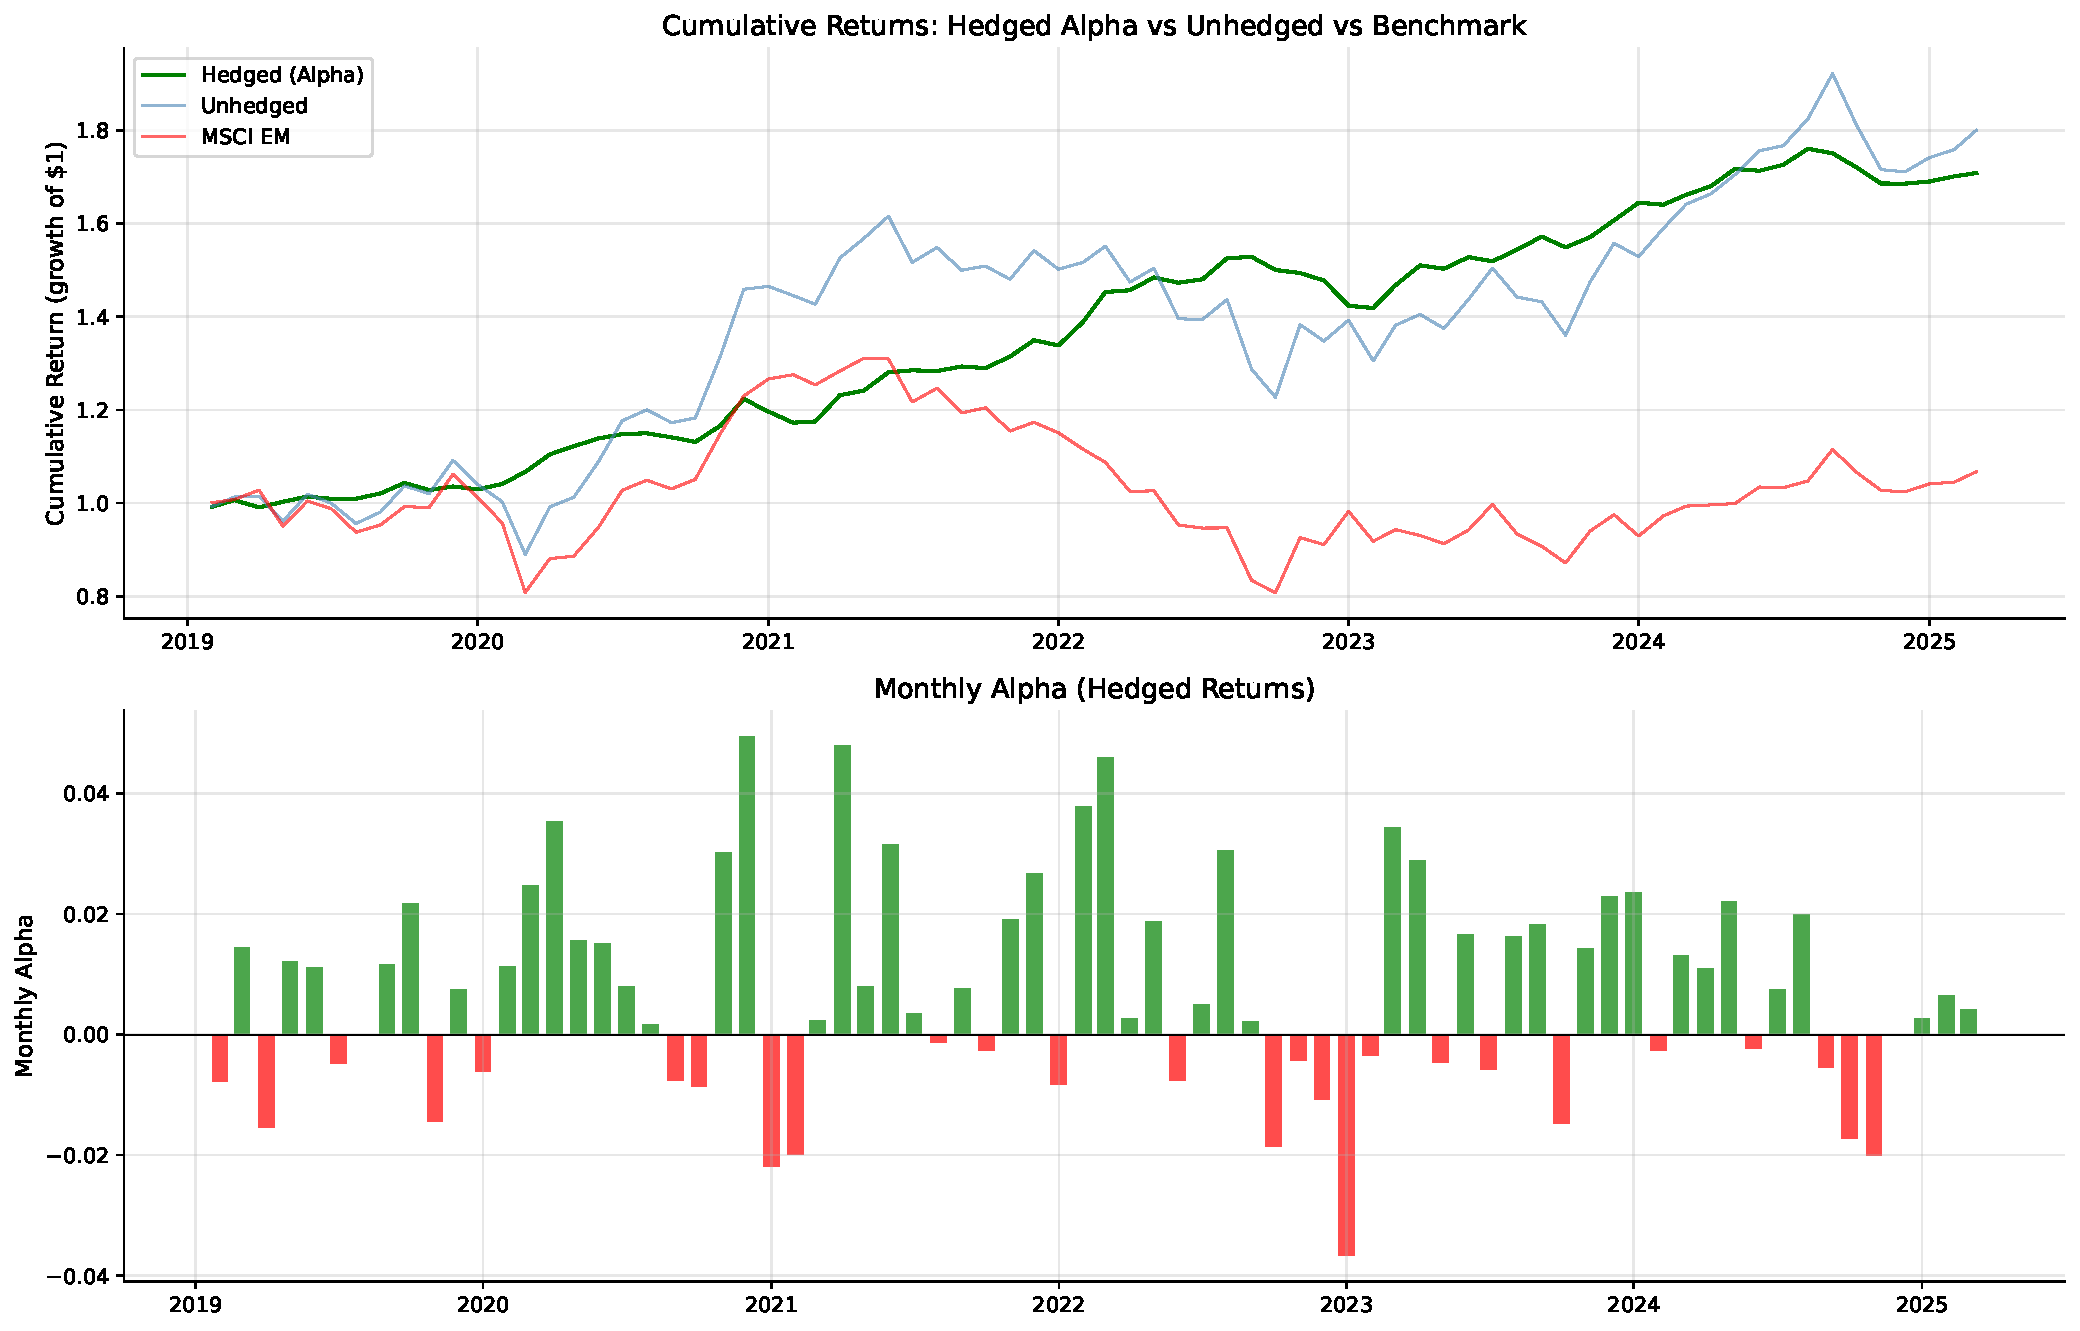
\includegraphics[width=0.85\textwidth]{nb09_alpha_timeseries.pdf}
    \caption{Cumulative returns: hedged A6+Momentum (green), unhedged portfolio (blue), and MSCI EM benchmark (red), 2019--2025. The hedged strategy compounds at 8.9\% annually with a maximum drawdown of 7.2\%, versus 62.7\% for the benchmark.}
    \label{fig:cumulative}
\end{figure}

\subsection{Transaction Cost Analysis}

We model transaction costs as a linear function of portfolio turnover at both the stock and industry levels. Figure~\ref{fig:tc} plots the hedged Sharpe ratio as a function of round-trip cost assumptions under the uniform-cost specification. The break-even for maintaining a Sharpe ratio above 1.0 is 127 basis points, well above typical EM trading costs.

\begin{figure}[H]
    \centering
    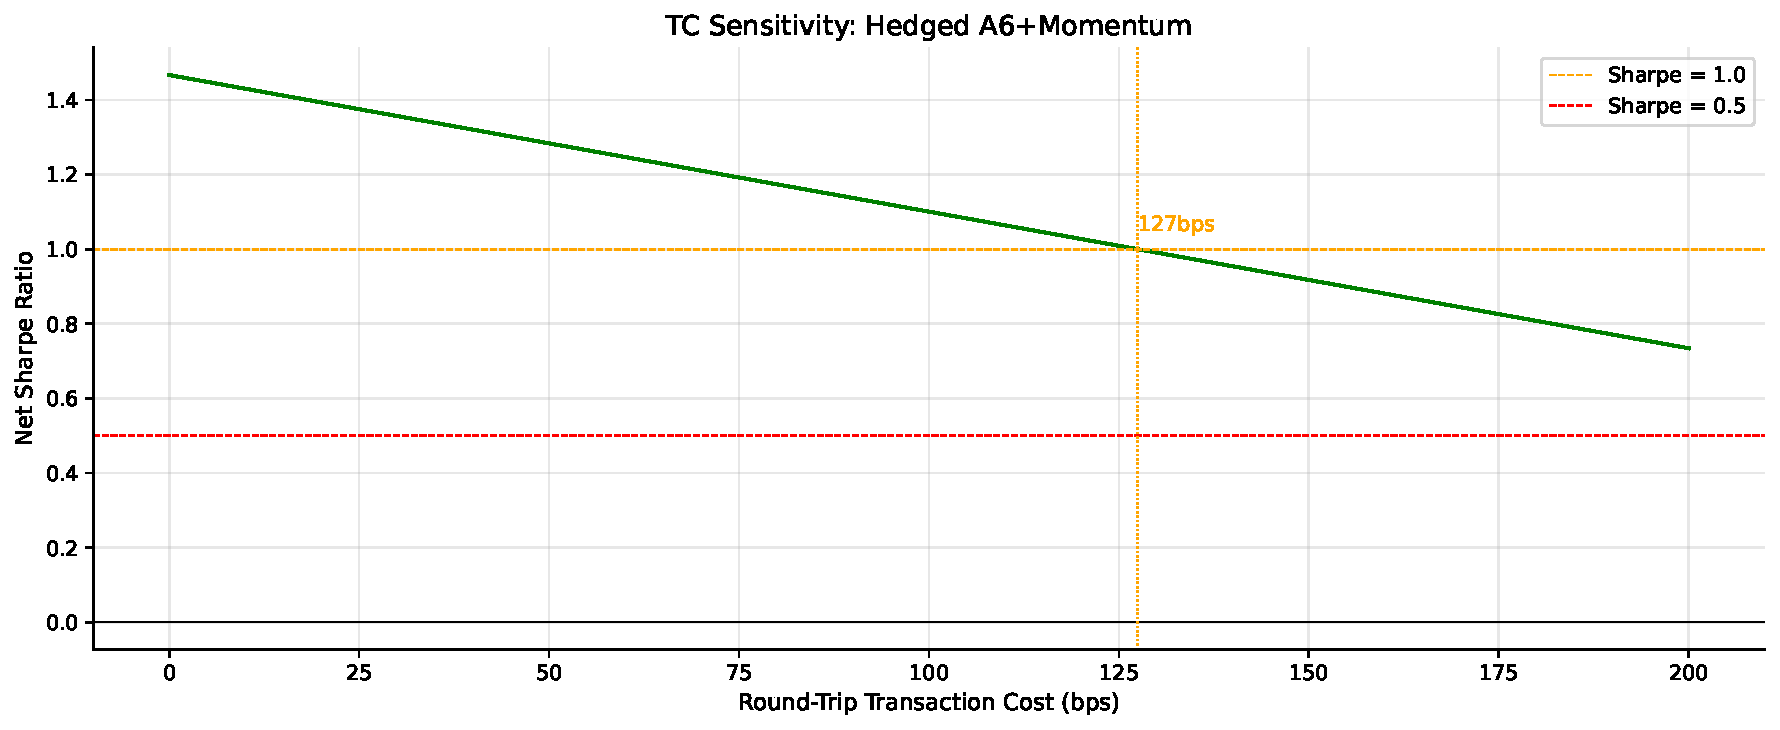
\includegraphics[width=0.80\textwidth]{nb09_tc_sensitivity.pdf}
    \caption{Transaction cost sensitivity of the hedged A6+Momentum strategy. The horizontal dashed line marks Sharpe = 1.0. The break-even transaction cost is 127 bps.}
    \label{fig:tc}
\end{figure}

To stress-test implementability, we also employ a country-weighted TC model based on \citet{domowitz2001}, assigning each stock a round-trip cost specific to its domicile country (e.g., Brazil 60 bps, China 50 bps, Hong Kong 20 bps, Egypt 70 bps). The resulting portfolio-weighted average is 44.6 bps---more than double the uniform 20 bps assumption. Under this conservative cost scenario, the hedged A6+Momentum Sharpe is 1.303, and the 127 bps break-even provides a 2.8$\times$ safety margin over the country-weighted average. Figure~\ref{fig:country_tc} illustrates the cross-country dispersion.

\begin{figure}[H]
    \centering
    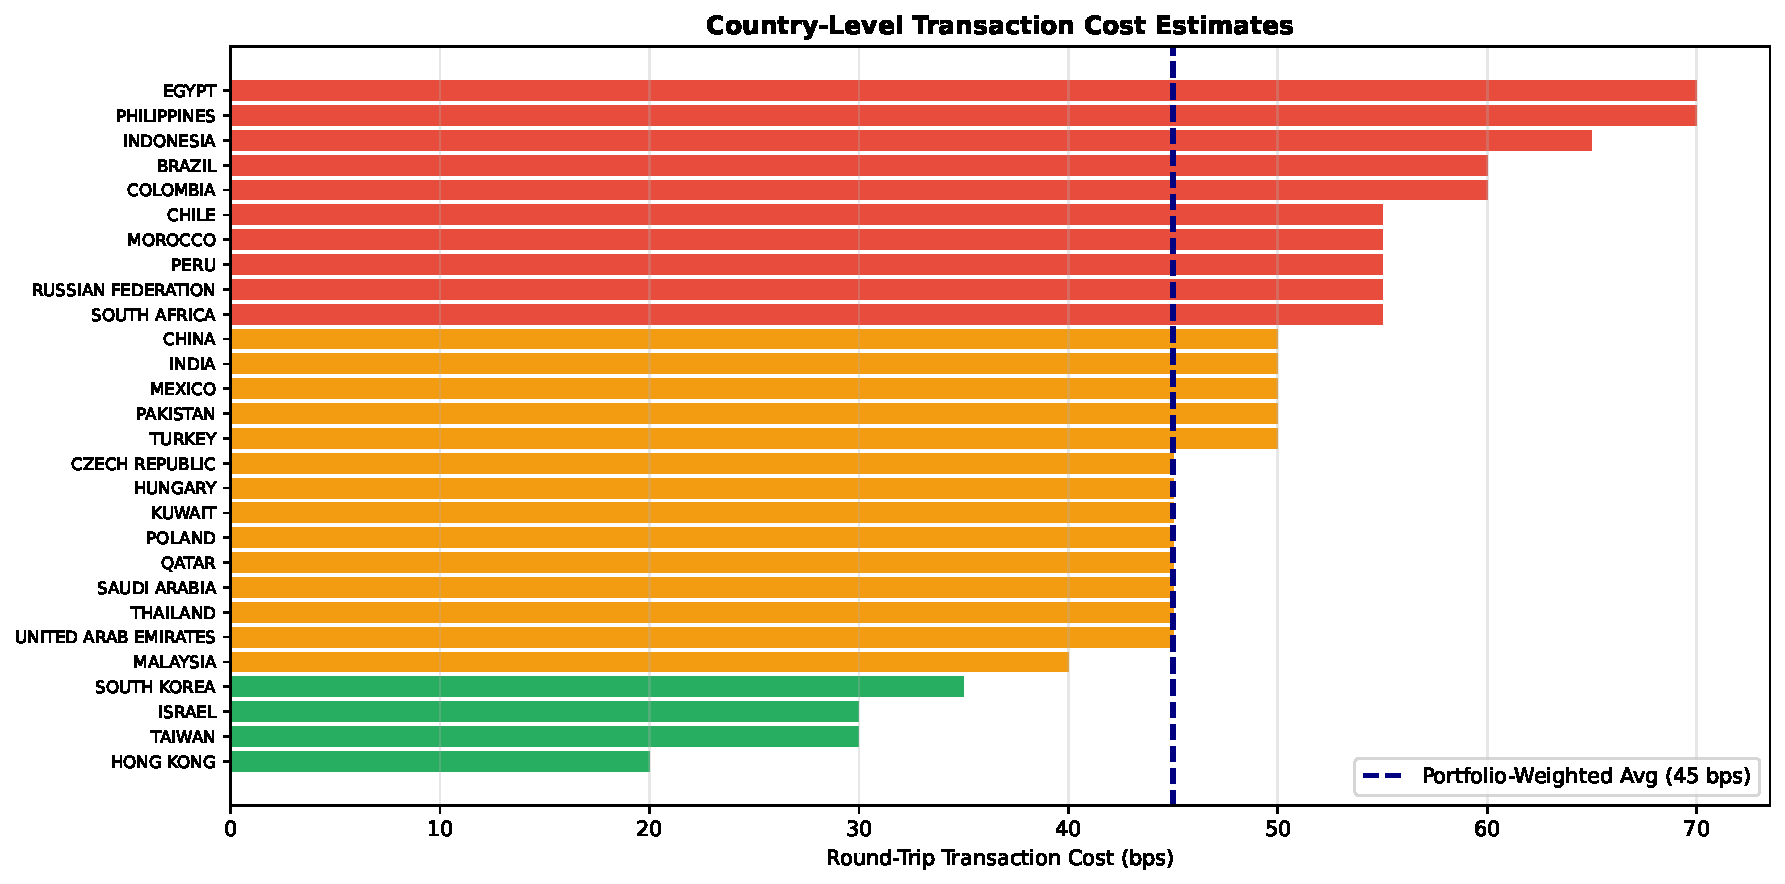
\includegraphics[width=0.80\textwidth]{country_tc_estimates.pdf}
    \caption{Country-level transaction cost estimates and the portfolio-weighted average (44.6 bps, dashed line).}
    \label{fig:country_tc}
\end{figure}


% ==================================================================
% 5. ROBUSTNESS TEST AND OTHER FINDINGS
% ==================================================================
\section{Robustness Tests and Other Findings}

\subsection{In-Sample versus Out-of-Sample Stability}

A key concern in factor strategy backtests is whether in-sample performance survives out-of-sample. We split the stock selection sample at January 2014, yielding 59 in-sample (2009--2013) and 135 out-of-sample (2014--2025) months. Table~\ref{tab:isoos} reports Sharpe ratios for each period.

\begin{table}[H]
\centering
\caption{In-Sample vs.\ Out-of-Sample Sharpe Ratios}
\label{tab:isoos}
\small
\begin{tabular}{lccc}
\toprule
\textbf{Strategy} & \textbf{IS Sharpe} & \textbf{OOS Sharpe} & \textbf{Retention} \\
\midrule
All6-EW     & 0.979 & 0.444 & 45\% \\
SF (best-1) & 0.930 & 0.414 & 45\% \\
Top3-EW     & 0.997 & 0.382 & 38\% \\
Corr03-EW   & 1.013 & 0.369 & 36\% \\
MSCI EM     & 0.689 & 0.142 & 21\% \\
\bottomrule
\end{tabular}
\begin{minipage}{0.92\textwidth}
\vspace{0.3em}
\footnotesize
\textit{Notes:} Retention = OOS Sharpe / IS Sharpe. IS = 2009--2013 (59 months); OOS = 2014--2025 (135 months).
\end{minipage}
\end{table}

All strategies exhibit IS-to-OOS degradation, as expected. All6-EW achieves the highest OOS retention rate (45\%) among the composite methods, consistent with its avoidance of estimation error. The benchmark itself retains only 21\%, indicating that the EM market environment changed substantially between the two periods---the factor strategies are more robust to this regime shift.

\subsection{Market Regime Analysis}

We split the hedged sample into months when the MSCI EM benchmark earned positive versus negative returns. The hedged A6+Momentum strategy generates positive average monthly alpha in both regimes: $+$0.94\% in EM up-months (41 months, 68\% hit rate) and $+$0.49\% in EM down-months (33 months, 58\% hit rate). The correlation between hedged returns and the benchmark is 0.07, confirming effective market neutrality. Alpha is not simply a leveraged market bet.

\subsection{Alpha Stability}

Annualized alpha is positive in every calendar year of the hedged sample: 3.9\% (2019), 16.9\% (2020), 10.1\% (2021), 9.3\% (2022), 8.6\% (2023), and 4.9\% (2024). The 2020 spike reflects strong factor performance during the COVID-19 recovery, when momentum and low-volatility stocks substantially outperformed. Rolling 24-month alpha remains positive in all periods, with the annual Sharpe ratio exceeding 0.9 in every full year.

\subsection{Country-Weighted Transaction Cost Robustness}

As a key robustness check, we compare strategy rankings under uniform (20 bps) versus country-weighted (44.6 bps) transaction costs. Table~\ref{tab:mf_tc_robust} reports TC-adjusted Sharpe ratios for all eight multi-factor variants.

\begin{table}[H]
\centering
\caption{Multi-Factor TC-Adjusted Sharpe Ratios}
\label{tab:mf_tc_robust}
\small
\begin{tabular}{lcccc}
\toprule
\textbf{Variant} & \textbf{Gross} & \textbf{20 bps} & \textbf{30 bps} & \textbf{50 bps} \\
\midrule
All6-EW     & 0.633 & 0.608 & 0.596 & 0.570 \\
All6-ICwt   & 0.616 & 0.597 & 0.587 & 0.567 \\
SF (best-1) & 0.594 & 0.578 & 0.570 & 0.555 \\
Top3-EW     & 0.600 & 0.574 & 0.561 & 0.535 \\
Corr03-EW   & 0.599 & 0.571 & 0.557 & 0.528 \\
Corr05-EW   & 0.580 & 0.551 & 0.537 & 0.508 \\
\bottomrule
\end{tabular}
\begin{minipage}{0.92\textwidth}
\vspace{0.3em}
\footnotesize
\textit{Notes:} All6-EW dominates at every TC level. The gap between All6-EW and alternatives widens at higher cost levels, confirming that its diversification benefit is not an artifact of ignoring costs. The country-weighted average of 44.6 bps falls between the 30 and 50 bps columns.
\end{minipage}
\end{table}

Under country-weighted costs, A6+Momentum's hedged Sharpe declines from 1.393 (at 20 bps) to 1.303 (at 45 bps), a reduction of 6.5\%. The strategy remains the only one exceeding Sharpe 1.0 under both cost assumptions (Table~\ref{tab:hedged}), confirming its implementability in realistic EM conditions.

\subsection{Covariance Estimation and Window Sensitivity}

Portfolio construction results are robust to the covariance estimator. Momentum-weighted and equal-weighted allocations are mechanically insensitive to covariance choice, while optimization-based methods (TO-MVO, Black-Litterman, minimum variance) show moderate sensitivity, with Ledoit-Wolf and sample covariance performing similarly and EWMA slightly worse. Results are also robust to estimation window length: 60-month windows generally produce slightly higher Sharpe ratios than 36-month windows.

\subsection{Look-Ahead Bias Audit}

We conducted a comprehensive audit of the entire pipeline. Data processing (winsorization, neutralization, imputation) uses only cross-sectional data at month $t$. Factor selection and covariance estimation use rolling windows ending at $t{-}1$. Stock selection at $t$ predicts returns at $t{+}1$. Beta hedging estimates $\hat{\beta}_t$ from $[t{-}60, t{-}1]$, excluding month $t$. No future information enters any stage of the pipeline. The IC is computed contemporaneously (factor at $t$ versus return at $t$), which is standard but may slightly overstate true predictive power; the backtest itself uses the correct one-month lag.

\subsection{Weight Concentration}

The Herfindahl-Hirschman Index (HHI) of momentum weights averages 0.131, compared to 0.091 for equal weighting, with a maximum of 0.211. No single industry ever exceeds approximately 20\% portfolio weight. This moderate concentration indicates that the strategy does not take extreme sector bets, maintaining broad diversification across all eleven industries.


% ==================================================================
% 6. CONCLUSION
% ==================================================================
\section{Conclusion}

This paper presents a comprehensive investigation of factor investing in emerging markets, tracing the full pipeline from factor evaluation through multi-factor composition, portfolio construction, and dynamic beta hedging. Five findings emerge.

First, all six canonical factors---size, value, quality, momentum, volatility, and dividend yield---carry cross-sectional predictive information in EM, though with signs that sometimes differ from developed-market premia. Second, equal-weighting all six factors dominates more complex composition methods out-of-sample, consistent with the theoretical result that estimation error makes naive diversification preferable to optimization \citep{demiguel2009}. Third, momentum-weighted cross-industry allocation outperforms nine alternative portfolio construction techniques by capturing industry-level momentum. Fourth, dynamic beta hedging converts a moderate long-only strategy (Sharpe 0.59) into a high-alpha market-neutral strategy (Sharpe 1.47, alpha 8.9\%, maximum drawdown 7.2\%). Fifth, these results are robust to realistic implementation costs: under country-weighted transaction costs of 44.6 bps \citep{domowitz2001}---more than double the typical uniform assumption---the net hedged Sharpe remains 1.30, and the break-even cost of 127 bps provides a 2.8$\times$ safety margin. Results are also insensitive to covariance estimators, estimation window lengths, and market regimes.

Two caveats apply. Our analysis is based on backtested, not live-traded, returns; market impact and implementation slippage may reduce realized performance, particularly for less liquid EM stocks. The hedged sample (74 months, 2019--2025) is relatively short, and the alpha may partially reflect favorable conditions for factor strategies during this period. Extensions to country-level factor models, dynamic factor timing, and alternative hedge instruments are natural directions for future research.


% ==================================================================
% BIBLIOGRAPHY
% ==================================================================
\newpage
\bibliographystyle{plainnat}
\bibliography{references}

\end{document}
